% Created 2016-02-10 Wed 14:16
\documentclass[presentation]{beamer}
\usepackage[utf8]{inputenc}
\usepackage[T1]{fontenc}
\usepackage{fixltx2e}
\usepackage{graphicx}
\usepackage{grffile}
\usepackage{longtable}
\usepackage{wrapfig}
\usepackage{rotating}
\usepackage[normalem]{ulem}
\usepackage{amsmath}
\usepackage{textcomp}
\usepackage{amssymb}
\usepackage{capt-of}
\usepackage{hyperref}
\usetheme{Warsaw}
\author{Justin Pounders}
\date{\today}
\title{The Neutron Spectrum}
\hypersetup{
 pdfauthor={Justin Pounders},
 pdftitle={The Neutron Spectrum},
 pdfkeywords={},
 pdfsubject={},
 pdfcreator={Emacs 24.5.1 (Org mode 8.3.2)}, 
 pdflang={English}}
\begin{document}

\maketitle

\begin{frame}[label={sec:orgheadline1}]{Review: SLBW Capture}
\begin{align*}
  \bar{\sigma}_x(E) = \sigma_0(E) \frac{\Gamma_{x,i}}{\Gamma_i} \psi(u,\alpha,\beta)
\end{align*}
where
\begin{align*}
  \psi(u,\alpha,\beta) &= \frac{1}{\beta\sqrt{\pi}}
                         \int_{-\infty}^\infty dv \frac{1}{1+v^2} \times \\
                       &\phantom{=}  \exp\left\{ -\frac{(v-u)^2}{\beta^2}
                         \left[ 1 - \frac{1}{2}\alpha(v-u) + \frac{5}{16}\alpha^2(v-u)^2 + \hdots \right] \right\}
\end{align*}
\begin{align*}
  \alpha = \frac{\Gamma_i}{2E}
  \quad \text{and} \quad
  \beta = \frac{2\Gamma_D}{\Gamma_i} = 4 \sqrt{\frac{E_i kT}{A}} \frac{1}{\Gamma_i} \;\;.
\end{align*}
\end{frame}
\begin{frame}[label={sec:orgheadline2}]{Review: SLBW Scattering}
\begin{align}
  \bar{\sigma}_e(E) = 4\pi a^2 + \sigma_0(E)\frac{2a}{\lambda}\phi(u,\alpha,\beta) + \sigma_0(E)\frac{\Gamma_{n,i}}{\Gamma_i}\psi(u,\alpha,\beta)
\end{align}
where
\begin{align}
  \phi(u,\alpha,\beta) &= \frac{1}{\beta\sqrt{\pi}}
                         \int_{-\infty}^\infty dv \frac{v}{1+v^2} \times \\
                       &\phantom{=} \exp\left\{ -\frac{(v-u)^2}{\beta^2}
                         \left[ 1 - \frac{1}{2}\alpha(v-u) + \frac{5}{16}\alpha^2(v-u)^2 + \hdots \right] \right\}
\end{align}
\end{frame}

\begin{frame}[label={sec:orgheadline3}]{Introduction}
\begin{block}{What is a neutron \emph{spectrum}?}
The neutron population depends on energy, \(n(E)\).  Multiplying by speed produces \(\phi(E) = v(E)n(E)\).  This is called the spectrum.
\end{block}
\end{frame}
\begin{frame}[label={sec:orgheadline4}]{Introduction}
\begin{block}{Classifying the neutron spectrum}
\begin{enumerate}
\item Fission range (\(E > 0.5 \text{ MeV}\))
\item Slowing-down range (\(1 \text{ eV} < E < 50 \text{ keV}\))
\item Thermal range (\(E < 1 \text{ eV}\))
\end{enumerate}
\end{block}
\end{frame}
\begin{frame}[label={sec:orgheadline5}]{Introduction}
\begin{figure}
  \centering
  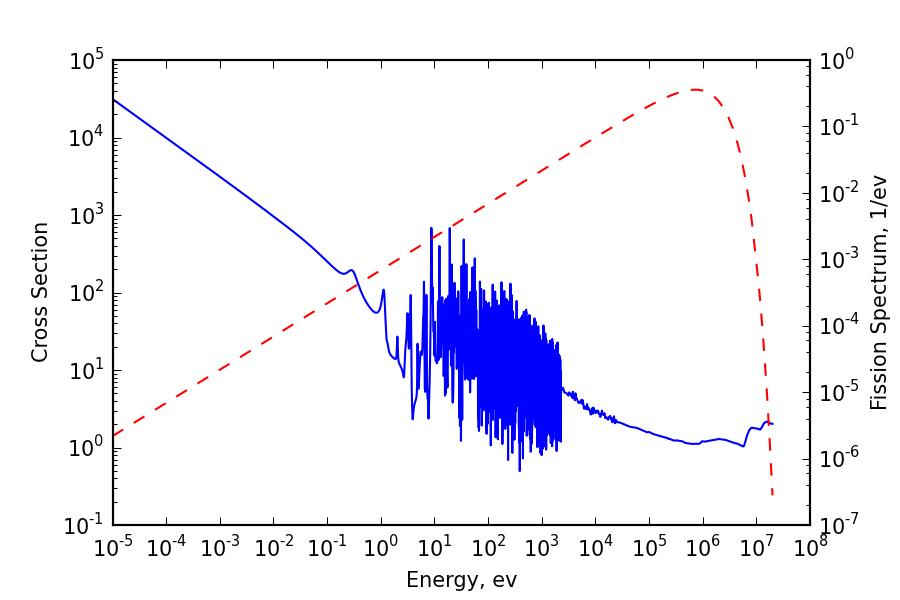
\includegraphics[width=0.75\textwidth]{../notes/u235fission.png}
  \caption{Fission cross section (blue) and fission spectrum (red) of uranium-235.}
  \label{fig::u235fission}
\end{figure}
\end{frame}
\begin{frame}[label={sec:orgheadline6}]{Fission Energy Range}
\begin{itemize}
\item Highest energy range
\item \(E > 0.5 \text{ MeV}\)
\item Neutrons created from fission
\end{itemize}
\begin{align*}
\phi(E) dE \approx \frac{\chi(E)}{\Sigma_t(E)} \times \text{ constant}
\end{align*}
\end{frame}
\begin{frame}[label={sec:orgheadline7}]{Slowing-Down Range}
\begin{itemize}
\item Intermediate (epi-thermal) energy range
\item \(1 \text{ eV} < E < 50 \text{ keV}\)
\item Resonances live here
\item Interactions dominated by elastic scattering and resonance absorption
\end{itemize}
\begin{align*}
  \phi(E) &= \frac{\left[ \Sigma_a(E_1) + \Sigma_s^H \right] E_1 \phi(E_1)}{\left[ \Sigma_a(E) + \Sigma_s^H \right] E} \times \\
          &\phantom{=}  \exp\left[ -\int_E^{E_1} \frac{\Sigma_a(E')}{\left[ \Sigma_a(E') + \Sigma_s^H \right] E'} dE' \right].
\end{align*}
\end{frame}
\begin{frame}[label={sec:orgheadline8}]{Thermal Range}
\begin{itemize}
\item Low energy range
\item \(E < 1 \text{ eV}\)
\item Neutrons in thermal equilibrium with medium
\item Few if any resonances
\item Characterized by Maxwell-Boltzmann dist. with effective temperature
\end{itemize}
\begin{align*}
  \phi(E) = 2 \sqrt{\frac{E}{\pi}} \left( \frac{1}{kT} \right)^{3/2} \exp\left( - \frac{E}{kT} \right).
\end{align*}
\end{frame}
\begin{frame}[label={sec:orgheadline9}]{Characteristic Neutron Spectrum}
\begin{figure}
  \centering
  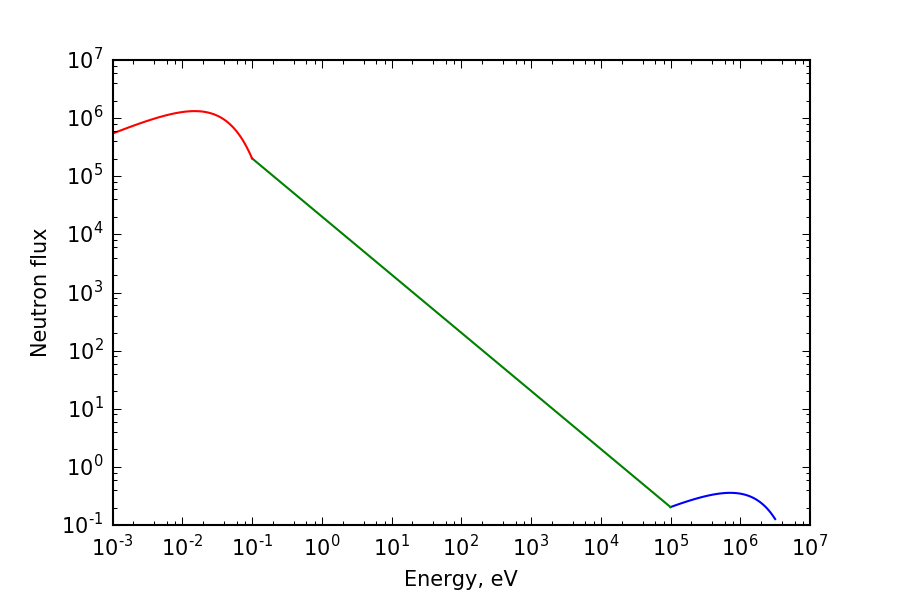
\includegraphics[width=0.75\textwidth]{../notebooks/spectrumcartoon.png}
  \caption{Rough caricature of a typical neutron spectrum.}
  \label{fig::spectrum}
\end{figure}
\end{frame}
\begin{frame}[label={sec:orgheadline10}]{Slowing Down and Resonance Absorption}
\begin{figure}
  \centering
  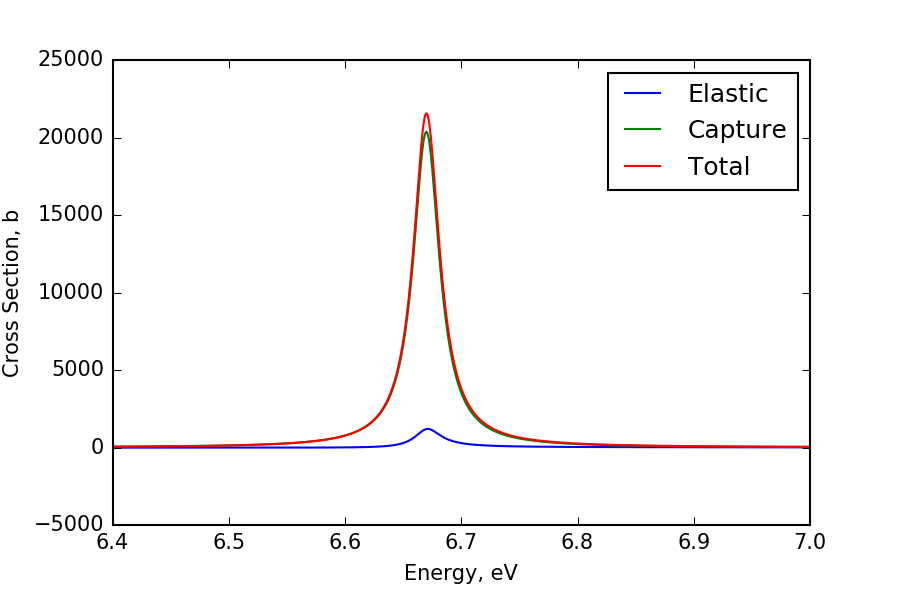
\includegraphics[width=0.75\textwidth]{../notebooks/xs0.png}
  \caption{Resonance cross section at 0K.}
\end{figure}
\end{frame}
\begin{frame}[label={sec:orgheadline11}]{Slowing Down and Resonance Absorption}
\begin{figure}
  \centering
  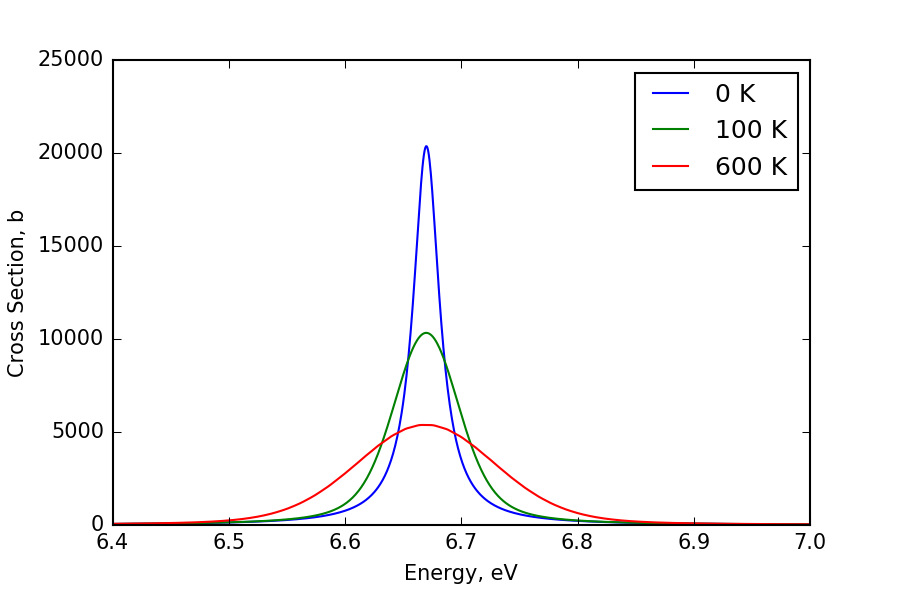
\includegraphics[width=0.75\textwidth]{../notebooks/capture_broad.png}
  \caption{Doppler broadening of capture resonance.}
\end{figure}
\end{frame}

\begin{frame}[label={sec:orgheadline12}]{Slowing Down and Resonance Absorption}
\begin{figure}
  \centering
  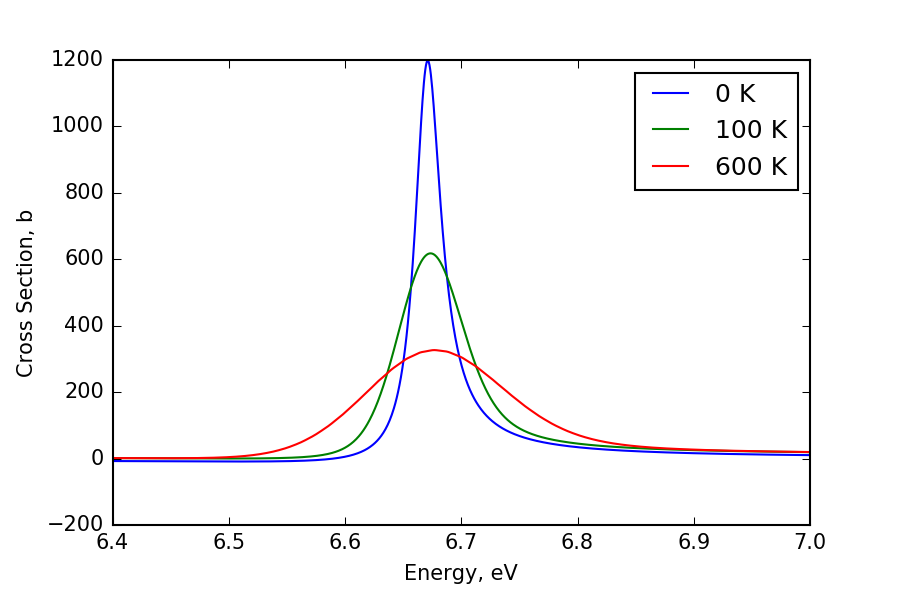
\includegraphics[width=0.75\textwidth]{../notebooks/scatter_broad.png}
  \caption{Doppler broadening of scatter resonance.}
\end{figure}
\end{frame}

\begin{frame}[label={sec:orgheadline13}]{Slowing Down and Resonance Absorption}
\begin{figure}
  \centering
  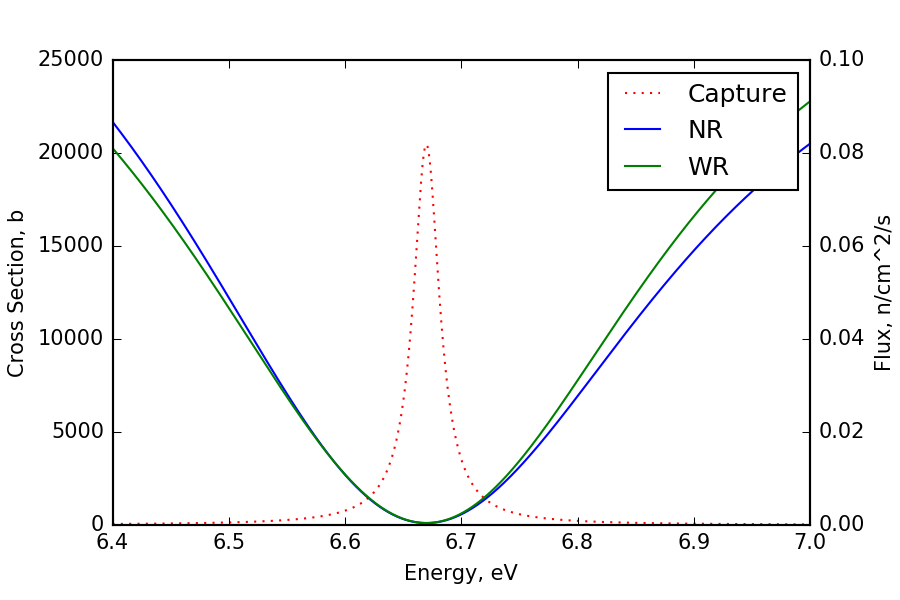
\includegraphics[width=0.75\textwidth]{../notebooks/selfshielding.png}
  \caption{Self shielding of neutron flux in resonance.}
\end{figure}
\end{frame}

\begin{frame}[label={sec:orgheadline14}]{Slowing Down and Resonance Absorption}
\begin{figure}
  \centering
  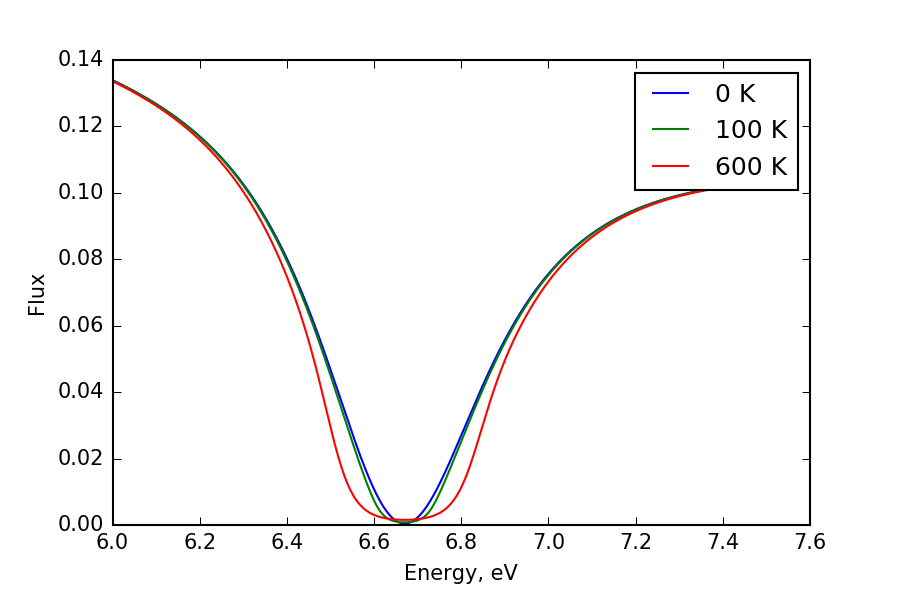
\includegraphics[width=0.75\textwidth]{../notebooks/selfshielding_broadZoom.png}
  \caption{Self shielding of neutron flux in resonance.}
\end{figure}
\end{frame}
\end{document}